% main.tex: camera-ready of "How Much Dependency Can a Marginal Rule See?" (DiffuLM @ NeurIPS 2026).
% Tables in tables/ and figures in figures/ are generated by scripts/report/.
\documentclass{article}
\usepackage[dblblindworkshop, final, nonatbib]{neurips_2026}
\workshoptitle{Diffusion Language Models: Foundations, Efficiency, and Reasoning (DiffuLM)}

\usepackage[utf8]{inputenc}
\usepackage[T1]{fontenc}
\usepackage[hidelinks]{hyperref}
\usepackage{url}
\usepackage{booktabs}
\usepackage{amsfonts}
\usepackage{amsmath,amssymb}
\usepackage{nicefrac}
\usepackage{microtype}
\usepackage{xcolor}
\usepackage{graphicx}
\usepackage{caption}
\captionsetup{font=small}

% float-only pages centre their floats vertically by default, which leaves an
% appendix table stranded in the middle of an otherwise empty page.
\makeatletter\setlength{\@fptop}{0pt}\makeatother

\newcommand{\C}{\mathrm{C}}
\newcommand{\given}{\,\vert\,}
\newcommand{\Chat}{\widehat{\C}}

\title{How Much Dependency Can a Marginal Rule See?\\
Total Correlation in Diffusion LM Parallel Decoding}

\author{%
  \mdseries Dovud Asadov \quad Rustambek Urokov \quad Qobiljon Toshnazarov\\
  Kayumov Abduaziz \quad Mardon Hazratov \quad Husanboy Mansuraliyev\\
  New Uzbekistan University\\
  {\footnotesize\texttt{\{d.asadov, r.urokov, q.toshnazarov, a.kayumov, m.hazratov, h.mansuraliyev\}@newuu.uz}}
}

\begin{document}
\maketitle

\begin{abstract}
A masked diffusion language model commits several masked positions per step. When its
conditionals compose into a joint, the exact cost of committing a set $S$ is that joint's
conditional total correlation $\C(S\given c)$. When they do not, we say exactly what our
estimate measures. Many systems choose the commit set from per-position marginals. That
such a rule cannot \emph{determine} $\C$ is elementary, and we state it exactly: the
marginals certify $\C\le W=B-\max_i H(Y_i)$, with $B$ the summed marginal entropy, and at
fixed marginals $\C$ takes every value up to a maximum $\C_{\max}\le W$. We ask instead
how well the marginals \emph{predict} an order-averaged estimate $\Chat$ of $\C$, per
candidate set on four masked diffusion LMs from two families, $247$ to $516$ blocks per
model and regime. Outside Dream-instruct, a marginal-only predictor scored out-of-fold
and corrected for estimator variance leaves a residual of $0.74$ to $1.17$ bits, $1.8$
to $3.7$ times below a reference that knows the marginal entropies but not the coupling.
Most of that predictability is the window itself. On a subset, $\Chat$ ranks blocks like
the KL cost of a parallel commit but sits a median $0.4$ to $1.1$ bits below it on prose
and in the deployed regime. Dream-instruct is the exception, mainly on prose, where its
conditionals are least self-consistent and the estimate stops measuring a commit cost. These results concern predicting $\C$ for a fixed set, not the gain of a
decoder that coordinates its commits. Getting there requires a validated readout. Dream
and LLaDA need \emph{opposite} logit-position conventions, and reading Dream with the
wrong one costs $6.9$ bits on the correct token, inflates a conditional-inconsistency
diagnostic $14$ to $41\times$, and in the deployed regime erases the confidence-error
correlation on Dream-base and reverses it on Dream-instruct. We specify gates that
measure the convention and report them for every checkpoint. Scoring six marginal rules
against measured $\C$, pooling across the block beats gating on its weakest position in
all $24$ paired comparisons, and the top-2 margin, which dominates confidence on tasks
with analytic $\C$, does not on these checkpoints.
\end{abstract}

\section{Introduction}
\label{sec:intro}

A masked diffusion language model (dLLM) \cite{llada,dream} writes text by committing
several masked positions per denoising step, and that parallelism is the entire source
of its speed. Which positions to commit is therefore the central control decision, and a
large body of work answers it with a rule computed from each position's marginal
separately: token confidence \cite{fastdllm,dynamicdllm}, the top-2 margin, the
predictive entropy, or cross-step stability \cite{less,stability}. A second line
estimates the dependency itself, usually from attention \cite{dapd,geoblock}.

The cost these rules are approximating is known exactly. Committing a set $S$ in one
step samples each position from its own marginal and discards the joint structure, and
the Kullback--Leibler cost of that factorization is the \emph{conditional total
correlation}
\begin{equation}
  \C(S \given c) \;=\; \sum_{i \in S} H(Y_i \given c) \;-\; H(Y_S \given c) \;\ge\; 0,
  \label{eq:tc}
\end{equation}
the information shared among the positions of $S$ given the already-decoded context $c$
\cite{parallelbench,dcd}. It is zero exactly when the positions are conditionally
independent, and it lower-bounds the achievable KL of a parallel commit
\cite{parallelbench,huang}.

That a marginal rule cannot \emph{determine} $\C$ is not news: it is stated in
\cite{cocommit}, motivates several decoders \cite{coherent,demask,dos}, and in the worst
case takes two lines of information theory, which \S\ref{sec:worstcase} states exactly as
a reference point. But the
worst case is not the question a practitioner has, since a decoder only meets the joints
a trained model produces. The open question, and the one we answer, is:

\begin{quote}
\emph{On a real dLLM, how much of the variation in $\C$ is recoverable from the
marginals, and how much do the rules that read them leave behind?}
\end{quote}

Answering it needs two things the literature has not put together: $\C$ measured per
candidate set on a real checkpoint, and a readout of that checkpoint one can trust.

\paragraph{Reading a dLLM's marginals is not trivial, and getting it wrong is not
loud.} Dream \cite{dream} keeps the shift of the autoregressive backbone it was
initialised from, so its hidden state at $i$ predicts the token at $i{+}1$. LLaDA
\cite{llada} predicts masked tokens in place. Two of the most widely used open
checkpoints require \emph{opposite} conventions, and the difference is invisible to any
type check. Reading Dream at $\delta{=}0$ costs $6.9$ bits on the correct token.
Its greedy decodes then collapse into a repeated token, but a measurement
pipeline that never decodes text sees none of that, and the confidence-error
correlation it reports is erased or reversed without looking wrong (\S\ref{sec:bugimpact}). We therefore specify three gates that \emph{measure} the
convention rather than assuming it.

\paragraph{Contributions.} \textbf{(1)} A measurement protocol with three gates
(\S\ref{sec:protocol}), namely readout offset, forward-pass determinism, and a
decode-and-read check. The offset gate scores \emph{hidden} true tokens, so a
bidirectional model cannot pass by copying, and it recovers each checkpoint's documented
convention without being told it. \textbf{(2)} A single-variable ablation of what a
wrong readout does to the measurement (\S\ref{sec:bugimpact}). \textbf{(3)} $\C$
estimated per candidate set on four checkpoints, with the residual left by the
strongest marginal-only predictor we could fit, scored out-of-fold and corrected for
estimator variance, and a precise account of what the estimate means when the
conditionals do not compose (\S\ref{sec:explains}). \textbf{(4)} All six deployed rules
against measured $\C$, with paired tests (\S\ref{sec:fidelity}). As a reference point we
state the worst case exactly (\S\ref{sec:worstcase}), a short characterisation built on
the factorisation bound of \cite[Thm.~1]{huang} and the analysis of
\cite[\S4]{parallelbench}.

\section{Background and related work}
\label{sec:bg}

\paragraph{Masked diffusion decoding.} A masked dLLM's one-step kernel over the masked
positions factorises, $p_\theta(x_{t-1}\given x_t)=\prod_i p_\theta(x^i_{t-1}\given
x_t)$, a mean-field product \cite{mdlm,md4}. A decoder reveals a subset $S$ per step,
sampling each position from its marginal, and $|S|=1$ recovers any-order
autoregression.

\paragraph{Total correlation as the cost of parallelism.} That $\C$ governs
parallel-commit error is established from several directions: a KL floor
\cite{parallelbench,huang}, the dependency a factorised step drops \cite{dcd},
sequence-error step-scaling \cite{feng}, optimal-schedule analysis \cite{schedules},
convergence rates in $\C$ and its dual \cite{intrinsicdep}, an information-theoretic
separation of generation order from parallelisation bias \cite{genorder}, and a
Gaussian-field analysis \cite{gaussiantc}. Dataset-level estimation dates to
non-autoregressive translation \cite{huang}. ParallelBench \cite{parallelbench} supplies
the synthetic family with analytic $\C$ that we reuse in \S\ref{sec:worstcase}, and
finds that a confidence rule loses to random selection there once $\C>0$. We add a per-candidate-set estimate
of $\C$ on real checkpoints and ask how much of it the marginals recover.

\paragraph{Dependency-aware decoding.} Many recent decoders replace confidence with an
estimated dependency signal: attention-derived graphs \cite{dapd,geoblock,clad},
learned pairwise mutual information \cite{neuralmi}, dependency predictors
\cite{demask,dawn,dos}, mean-field coordination \cite{meanfield}, conditional
independence testing \cite{punt}, local coherence \cite{locallycoherent}, a learned
commitment policy \cite{tracelock}, and a coordination pass that names $\C$ as the
obstacle \cite{cocommit}. We measure how well the marginals predict the dependency of a
fixed candidate set, not how much a decoder that coordinates its commits would gain, which
needs a matched-compute comparison that we do not run.

\paragraph{Conditional inconsistency in masked models.} That an MLM's conditionals need
not compose into any joint is long established \cite{mlminconsist}, with consequences
for sampling dynamics \cite{glauber} and denoising order \cite{pathdenoise}. The
specific diagnostic we use as a covariate, which holds the assignment fixed and varies
the reveal order so that a consistent joint gives exactly zero spread, is
\emph{chain-rule deviation}, introduced for order-agnostic LMs by \cite{chainruledev}.
We do not claim it, and report it as a covariate that \S\ref{sec:bugimpact} shows is
highly sensitive to a readout error.

\section{The worst case: what a marginal profile certifies}
\label{sec:worstcase}

Since $H(Y_S\given c)\ge0$, Eq.~\eqref{eq:tc} gives immediately
\begin{equation}
  0 \;\le\; \C(S\given c) \;\le\; \sum_{i\in S} H(Y_i\given c) \;=:\; B(S\given c),
  \label{eq:budget}
\end{equation}
so the summed marginal entropy is a \emph{certified upper bound} on the dependency a
parallel commit discards. A tighter ceiling that depends on the marginals only through
their entropies is $\C\le W:=B-\max_i H(Y_i\given c)$, since a joint is never less
uncertain than its most uncertain coordinate, and it shows exactly when the marginals
settle the question: they certify $\C=0$ if and only if at most one position of $S$ is
uncertain.

The set of joints with a fixed marginal profile (a transportation polytope) is convex
and compact, and always contains the product measure, so $\C=0$ is attainable. At the
other end a minimum-entropy coupling gives $\C_{\max}=B-\min_P H(P)$, and since
$H(P)\ge\max_i H(Y_i)\ge B/k$,
\begin{equation}
  \C_{\max} \;\le\; W \;=\; B-\max_i H(Y_i) \;\le\; (1-1/k)\,B ,
  \label{eq:width}
\end{equation}
with equality throughout, $(k{-}1)H(Y_1)$, for an equal-marginal profile, attained by
the comonotone coupling. Because $\C$ is continuous on a connected set, every intermediate value is
realised. Minimising the concave $H$ over a polytope attains its minimum at a vertex, so
for small $k$ we verify $\C_{\max}$ by exact vertex enumeration: $k$ fair bits span
exactly $[0,k{-}1]$ bits (Table~\ref{tab:nontightness}).

A clean witness is $n$ fair coins against $n$ coins conditioned on exactly $n/2$ heads:
identical marginals and $B=n$ bits, but $\C=n-\log_2\binom{n}{n/2}$ ($1.415$ bits at
$n{=}4$), so every marginal rule must score them identically \cite{marginalsmatch}.


\subsection{An exact audit, and why a benchmark result cannot settle this}
\label{sec:oracle}

To score the deployed rules where $\C$ is known exactly we use the synthetic
list-operation family of ParallelBench \cite{parallelbench} and its analytic $\C$, plus
two controls of our own. Enumerated and closed-form $\C$ agree to $1.6\times10^{-14}$
bits. Over the $355$ candidate sets, the six rules collapse to four distinct rankings and
the top-2 margin ranks $\C$ far better than confidence, by $0.394$ $[0.296,0.494]$ under
a paired bootstrap of the difference (Table~\ref{tab:proxy}). The bootstrap is paired
because the rules score the \emph{same} sets.

Every proxy attains a perfect safe-set AUROC of $1.000$ here, and that number is empty:
on this family $\C=0$ holds \emph{if and only if} $B=0$, so any certainty detector scores
perfectly. We therefore treat the ranking above as a hypothesis to test on the four
checkpoints rather than a prescription, and \S\ref{sec:fidelity} finds it reverses.


\paragraph{Why this is a reference point and not a result.} Eq.~\eqref{eq:width}
quantifies over all joints compatible with a profile, not over the ones \emph{a
particular trained model} produces, which is what a decoder faces.
\S\ref{sec:explains} measures that.

\section{A measurement protocol for dLLM marginals}
\label{sec:protocol}

Everything in \S\ref{sec:explains} and \S\ref{sec:fidelity} rests on one contract:
given a masked canvas and a position $p$, return $p_\theta(Y_p \given \text{canvas})$.
Three gates establish that contract per checkpoint before any number is produced.

\paragraph{The estimator.} $\C$ needs the joint entropy $H(Y_S\given c)$, which is not
directly available, whereas the marginal terms are. We estimate it by the chain rule along
randomly sampled reveal orders. For a permutation $\pi$ of $S$ we draw one ancestral
path through the model's any-order conditionals and accumulate the \emph{exact} entropy
of each predicted categorical,
\begin{equation}
  \hat H_{\pi}(Y_S\given c) \;=\; \sum_{t=1}^{|S|}
  H_\theta\!\big(Y_{\pi(t)} \given y_{\pi(<t)}, c\big),
  \qquad
  y_{\pi(t)} \sim p_\theta\!\big(\cdot \given y_{\pi(<t)}, c\big),
  \label{eq:meter}
\end{equation}
and average over $M$ independent orders:
\begin{equation}
  \Chat_M(S\given c) \;=\; \underbrace{\sum_{i\in S} H_\theta(Y_i\given c)}_{B(S\given c)}
  \;-\; \frac{1}{M}\sum_{m=1}^{M}\hat H_{\pi_m}(Y_S\given c).
  \label{eq:chat}
\end{equation}
If the conditionals compose into a joint, the chain rule makes $\hat H_\pi$ unbiased for
$H(Y_S\given c)$ for \emph{any} single order, so averaging only reduces variance. We take
$M{=}64$ throughout, report the per-block
standard error $\mathrm{sd}_m(\hat H_{\pi_m})/\sqrt{M}$, and correct for it wherever
$\Chat$ enters a variance decomposition. The estimator queries the model only through
conditionals, so the identical code runs on the exact oracle of \S\ref{sec:oracle},
where it recovers analytic $\C$ to $0.0087$ bits, and on a checkpoint. Cost is $M|S|$
conditional queries per set, batched across orders.

\paragraph{What $\Chat$ estimates when the conditionals do not compose.} Let $q_\pi$ be
the joint over $S$ produced by revealing $S$ in order $\pi$ with the model's conditionals,
$\bar q=\mathbb{E}_\pi q_\pi$ the joint of a sampler whose order is uniformly random, and
$p_i$ the parallel marginals. Each $\hat H_\pi$ is unbiased for $H(q_\pi)$ whatever the
conditionals, so $\mathbb{E}\Chat_M=B-\mathbb{E}_\pi H(q_\pi)$. The cost of a parallel
commit relative to these samplers obeys the exact identity
\begin{equation}
  \mathbb{E}_\pi\,\mathrm{KL}(q_\pi\,\|\,\textstyle\prod_i p_i)
  \;=\;\mathrm{KL}(\bar q\,\|\,\textstyle\prod_i p_i)\;+\;I(\pi;Y_S),
  \label{eq:orderinfo}
\end{equation}
where $I(\pi;Y_S)\le\log_2 k!$ is the information the reveal order carries about the
outcome. When the conditionals compose, all three of $\mathbb{E}\Chat_M$, the left side
and the first term on the right equal $\C$, and $I(\pi;Y_S)=0$. When they do not, the
three separate. If every $q_\pi$ keeps the parallel marginals, $\mathbb{E}\Chat_M$ is the
left side, and it exceeds the cost relative to a random-order sampler by the order
information. Two fair bits show the gap: if one order makes the second bit agree with
the first with probability $0.9$ and the other makes it disagree with probability $0.9$,
each order gives $0.531$ bits while the mixture is uniform and costs nothing. If the
$q_\pi$ do not keep the parallel marginals, $\Chat$ is not a divergence at all and can
be negative. We measured both terms of \eqref{eq:orderinfo} directly on a subset
(App.~\ref{app:probe}). On its random blocks the per-order KL cost, the left side,
exceeds $\Chat$ by a median of $0.4$ to $1.1$ bits on LLaDA-base and Dream-base prose and
in their deployed regime, and $\Chat$ ranks blocks like it (Spearman $0.95$ and $0.90$,
pooled across settings). The residuals of \S\ref{sec:explains} are therefore residuals
for $\Chat$, not for the KL cost. On Dream-instruct prose the gap is $4.4$ and $5.6$ bits.

\paragraph{Gate 1: which logit index carries position $p$?} A dLLM's head need not be
aligned to its own positions. Dream keeps the shift of the autoregressive model it was
initialised from, so its hidden state at $i$ predicts the token at $i{+}1$
\cite{dream}, while LLaDA predicts masked tokens in place \cite{llada}. We do not take either
on faith. We mask the block, then score the log-probability the model assigns to the
tokens that were \emph{actually} there, reading at index $p+\delta$ for
$\delta\in\{-1,0,+1\}$. Because the true tokens are hidden, a bidirectional model cannot
win by copying: only the correct convention scores well. We require the winner to agree
at $k{=}1$ and $k{=}4$ and to beat the runner-up by at least one bit.

The gate recovers each model's documented convention without being told it, by margins
of $6.9$ to $11.0$ bits (Fig.~\ref{fig:gates}a, App.~\ref{app:gates}).

\paragraph{Gate 2: is the forward pass reproducible?} Two identical calls must return
identical logits. Our runs also required that scoring a sequence alone or in a batch move
no argmax, although batch composition moves log-probabilities by up to $0.56$
(App.~\ref{app:gates}). In the released gate the two batch shapes the estimator combines
must agree on every argmax and on $B$ to within $0.074$ bits RMS, a tenth of the
smallest residual we report. On a second GPU all four checkpoints pass with the two shapes
agreeing exactly, while scoring alone, which the measurement never does, flips $1$ of $64$
argmaxes on each Dream checkpoint (App.~\ref{app:probe}). We also assert that the first
sequentially decoded position, drawn from the parallel commit's distribution, never
disagrees with it, and count violations.

\paragraph{Gate 3: does it write?} We greedy-decode into an all-masked canvas using the
calibrated offset and read the output. At a wrong offset the decode collapses on all three
checkpoints we probed: one token fills $21$ to $32$ of $32$ prose positions, against runs
of at most $3$ at the calibrated offset (App.~\ref{app:probe}). The submitted gate only
required a non-empty decode, so the released code also requires a wrong offset to
produce such a collapse, and fails on any error.

\begin{figure}[t]
\centering
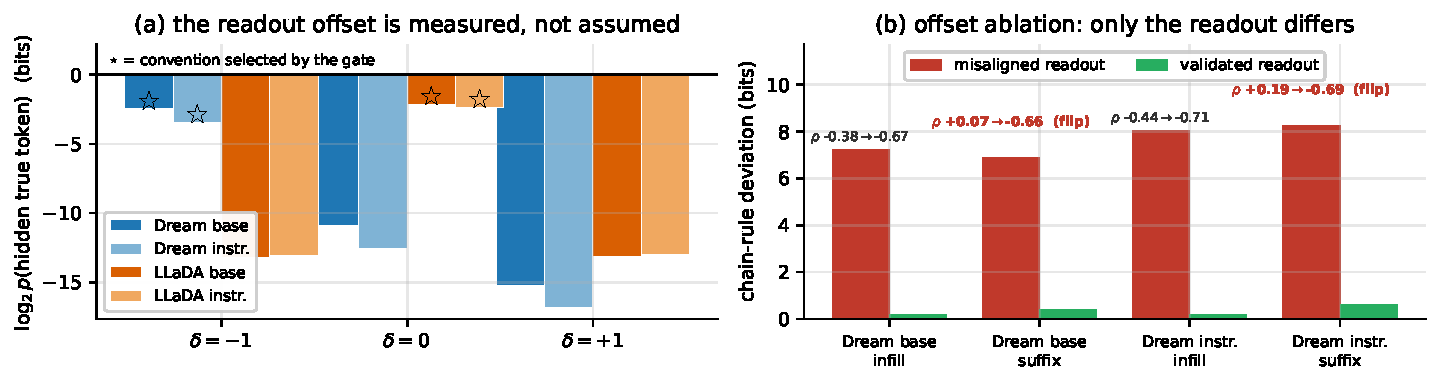
\includegraphics[width=\textwidth]{figures/fig1_gates.pdf}
\caption{\textbf{(a)} The offset gate. We mask a block and score the log-probability the
model assigns to the tokens that were actually there, reading at index $p+\delta$. The
truth is hidden, so a bidirectional model cannot win by copying. Stars mark the
convention the gate selects. Dream and LLaDA select \emph{opposite} conventions, each matching its own
documentation, without being told. \textbf{(b)} The offset ablation: identical corpus, blocks, reveal orders and code path, with only the readout changed. Chain-rule deviation
\cite{chainruledev} inflates $14$ to $41\times$ across both Dream checkpoints, and in the deployed regime the confidence-error correlation $\rho$ is erased on Dream-base and reversed on Dream-instruct.}
\label{fig:gates}
\end{figure}


\section{What a wrong readout manufactures}
\label{sec:bugimpact}

To measure what a misaligned readout costs we hold the corpus, blocks, reveal orders and
code path fixed and change only the offset, from the measured $-1$ to the naive $0$.
Three quantities move.

\emph{The consistency diagnostic.} Chain-rule deviation \cite{chainruledev}, exactly zero
for conditionals that compose into one joint, reads $6.9$ to $8.3$ bits under the
misaligned readout against $0.18$ to $0.59$ once corrected, across both Dream checkpoints
and both regimes: a factor of $14$ to $41$. Read naively, the misaligned number would
say that these checkpoints' conditionals are far from composing into a joint.

\emph{The headline correlation.} In the deployed regime the rank correlation between
confidence and parallel-decoding error reads $+0.07$ $[-0.06,0.19]$ and $+0.19$
$[0.07,0.31]$ under the misaligned readout, against $-0.66$ and $-0.69$ once corrected.
The misaligned readout erases the correlation on Dream-base and reverses it on
Dream-instruct. An earlier version of this work reported these numbers and concluded
that confidence is uninformative about parallel-decoding error in the deployed regime.
That conclusion came from the readout.

\emph{Total correlation itself.} Median $\Chat$ reads $-4.3$ and $-4.8$ bits under the
misaligned readout in the infill regime, against $+0.78$ and $+0.05$ corrected. Since
$\C\ge0$ for any genuine joint, a strongly negative estimate is impossible rather than
surprising, so the estimator flags the error that the disagreement metric hid.

\section{How much of $\C$ the marginals explain}
\label{sec:explains}

We apply \eqref{eq:chat} to $247$ to $516$ non-overlapping $k{=}4$ blocks per checkpoint
and regime, plus a $k{=}8$ replication, and ask how much of the resulting variation in
$\C$ a marginal-only predictor recovers. Predictors are scored out-of-fold with
document-grouped folds and corrected for the meter's own variance, which is $0.7$ to
$7.5\%$ of $\mathrm{Var}[\Chat]$. We sweep $k$-NN and ridge over five feature sets and
keep the best out-of-fold score (nested selection moves it by at most $0.035$ bits,
App.~\ref{app:nested}).

\paragraph{The marginals predict $\C$ well, mostly through the window they certify.}
The worst case \eqref{eq:width} confines $\C$ to $[0,\C_{\max}]\subseteq[0,W]$, with
median $W$ of $1.3$ to $10.8$ bits across settings, and Fig.~\ref{fig:explains}a shows
where real blocks fall inside $[0,W]$. Outside Dream-instruct, the best marginal-only predictor leaves a
residual of $0.74$ to $1.17$ bits (Table~\ref{tab:explains}). A window width and a residual
are different statistical objects, so we compare the residual with a reference that knows
the marginal entropies, hence $W$, but nothing about the coupling, with $\C$ uniform on
$[0,W]$. Knowing $\C_{\max}$, which top-$8$ profiles cannot give, would narrow it. The measured
residual is $1.8$ to $3.7$ times below that reference. Most of this predictability is the
window itself. Blocks with $W$ above one bit sit at a median of $0.44$ to $0.56$ of $W$, a one-parameter
predictor $f\cdot W$ matches the best predictor on LLaDA-base ($0.74$ and $1.07$ bits
against $0.74$ and $1.05$), and outside Dream-instruct, given $W$, the rank correlation
of any of the six rules with $\C$ lies between $-0.28$ and $+0.23$ (Table~\ref{tab:paired}). Outside
Dream-instruct the full profile adds most on Dream-base in the deployed regime, where it
lowers the residual from $1.81$ to $1.09$ bits.

\paragraph{Two families, one outlier, and where it comes from.} Six of the eight settings
agree closely. Dream-instruct is the exception ($1.62$ and $1.84$ bits), and the
exception is concentrated on prose. Under one pooled predictor its residual is $2.23$ and
$2.58$ bits on prose, above every other checkpoint's prose residual, and $0.92$ and
$1.28$ bits on code, its training domain (Table~\ref{tab:domain}). Its chain-rule
deviation on prose is the largest we measure. There the KL cost of a parallel commit exceeds
$\Chat$ by several bits (App.~\ref{app:probe}), so $\Chat$ does not measure it. It is not a generic
instruction-tuning effect, since LLaDA-instruct sits with the base checkpoints.

\paragraph{Robust to block size.} Repeating the measurement at $k{=}8$ on both base
checkpoints gives residuals of $1.60$ to $2.59$ bits, $3.4$ to $5.0$ times below the
coupling-agnostic reference, against $1.8$ to $3.7$ times at $k{=}4$
(Table~\ref{tab:k8}).

\paragraph{Where $\Chat$ leaves $[0,W]$.} No genuine joint gives $\C<0$ or $\C>W$. Beyond
two standard errors, $0\%$ to $25\%$ of blocks fall below zero and $0.4\%$ to $9.5\%$
above $W$. Outside Dream-instruct $79\%$ of these are hairlines within $0.2$ bits, $86\%$ of them on
code. There the per-block standard error under-covers: when the sampled paths nearly
coincide it is close to zero and misses the rare branches, so even the KL version, which
cannot be negative in expectation, falls below minus two standard errors on some of them
(App.~\ref{app:probe}). The substantive cases, beyond
$0.2$ bits, are $0.4\%$ to $5.9\%$ of blocks outside Dream-instruct and $8.1\%$ and
$14.6\%$ on it (Table~\ref{tab:domain}). We report these rates rather than clipping.
Excluding the blocks below zero moves Dream-instruct's residual from $1.62$/$1.84$ to
$1.19$/$1.57$ bits and leaves the other checkpoints essentially unchanged.

\begin{figure}[t]
\centering
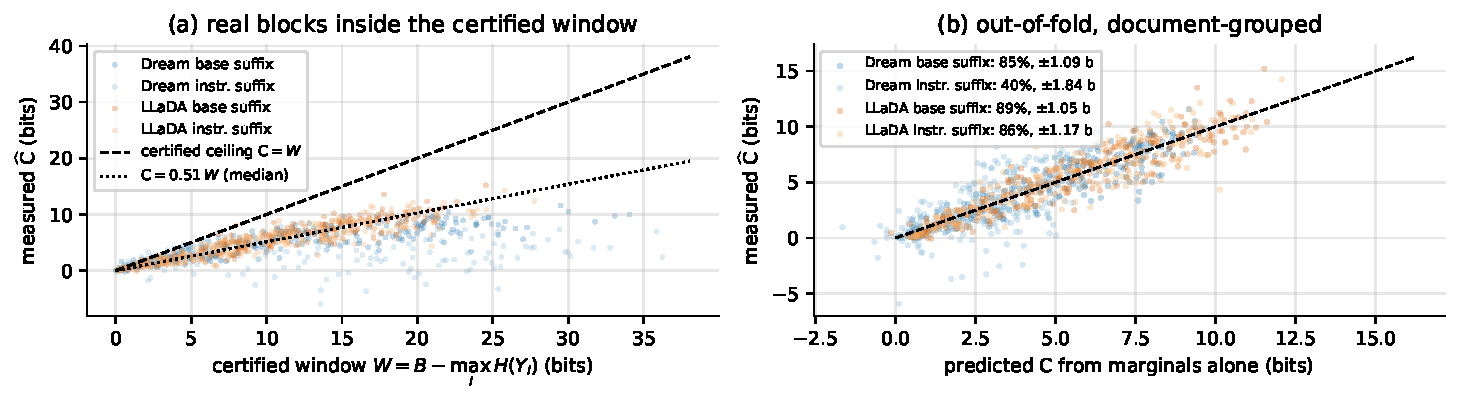
\includegraphics[width=\textwidth]{figures/fig2_explains.pdf}
\caption{\textbf{Deployed (suffix) regime only.} The infill settings are in
Table~\ref{tab:explains}. \textbf{(a)} Measured $\Chat$ against the certified window $W=B-\max_i H(Y_i)$ of \eqref{eq:width}. The dashed line is the ceiling $\C=W$ and the dotted line the median fraction of the window outside Dream-instruct. \textbf{(b)} The headline:
best marginal-only prediction of $\C$ against the truth, out-of-fold with
document-grouped folds. The scatter about the diagonal is the residual left by the
strongest marginal-only predictor we fit.}
\label{fig:explains}
\end{figure}

\begin{table}[t]
\centering
\small
\setlength{\tabcolsep}{4pt}
\caption{\textbf{How well the marginals predict $\mathrm{C}$.} $\mathrm{C}$ is estimated
per candidate set with the order-averaged chain-rule estimator, in bits. ``s.d.'' is the
block-to-block standard deviation after subtracting the estimator's own variance.
``\% Var'' is out-of-fold $R^2$ with document-grouped folds, corrected for estimator
variance, for a predictor built from the summed marginal entropy $B$ alone and for the
best of $40$ $k$-NN and ridge predictors over five feature sets up to the full top-$8$
profile, which subsumes every \emph{single-step} rule we score but not the cross-step
stability rules of \cite{less,stability}. The residual columns are noise-corrected
residual standard deviations: \emph{best} for that predictor (nested selection moves it
by at most $0.035$ bits, App.~\ref{app:nested}), \emph{$fW$} for the one-parameter
predictor $f\cdot W$ with $f$ fitted out-of-fold, and \emph{ref.} for a coupling-agnostic
reference that knows the marginal entropies, hence $W$, with $\mathrm{C}$ uniform on $[0,W]$.
$W=B-\max_i H(Y_i)$ is the certified window of \eqref{eq:width}, at the median block.}\label{tab:explains}
\begin{tabular}{lrrrrrrrrr}
\toprule
 & & \multicolumn{2}{c}{measured $\mathrm{C}$} & \multicolumn{2}{c}{\% Var$[\mathrm{C}]$} & \multicolumn{3}{c}{residual s.d. (bits)} & window \\
\cmidrule(lr){3-4}\cmidrule(lr){5-6}\cmidrule(lr){7-9}
Model / regime & $n$ & mean & s.d. & $B$ & best & best & $fW$ & ref. & $W$ \\
\midrule
Dream base / infill & $494$ & $1.70$ & $2.25$ & $65$ & $75$ & $1.13$ & $1.41$ & $2.04$ & $2.0$ \\
Dream base / suffix & $247$ & $4.90$ & $2.79$ & $81$ & $85$ & $1.09$ & $1.81$ & $4.06$ & $10.8$ \\
Dream instr. / infill & $494$ & $0.54$ & $1.89$ & $3$ & $26$ & $1.62$ & $2.03$ & $2.53$ & $1.3$ \\
Dream instr. / suffix & $247$ & $2.54$ & $2.37$ & $15$ & $40$ & $1.84$ & $3.59$ & $4.01$ & $6.7$ \\
LLaDA base / infill & $516$ & $1.78$ & $2.38$ & $86$ & $90$ & $0.74$ & $0.74$ & $1.52$ & $1.7$ \\
LLaDA base / suffix & $258$ & $5.47$ & $3.24$ & $88$ & $89$ & $1.05$ & $1.07$ & $3.48$ & $10.3$ \\
LLaDA instr. / infill & $516$ & $1.67$ & $2.28$ & $78$ & $85$ & $0.87$ & $0.95$ & $1.60$ & $1.6$ \\
LLaDA instr. / suffix & $258$ & $5.03$ & $3.13$ & $81$ & $86$ & $1.17$ & $1.34$ & $3.44$ & $9.5$ \\
\bottomrule
\end{tabular}
\end{table}


\section{Proxy fidelity on real checkpoints}
\label{sec:fidelity}

Table~\ref{tab:fidelity} scores all six marginal rules against measured $\C$. All $48$
model-regime-proxy correlations are negative and exclude zero under a
document-clustered bootstrap. That much is expected from $\C\le W$ once a rule tracks
certainty: given $W$, the correlations outside Dream-instruct fall to between $-0.28$ and
$+0.23$ (Table~\ref{tab:paired}). The informative part is how the rules compare with each other,
and two comparisons run against the synthetic audit.

\paragraph{Aggregation matters more than the statistic.} In every one of the eight
settings, pooling across the block beats taking its weakest position: confidence-mean
beats confidence-min, margin-mean beats margin-min, and summed neg-entropy beats maximum
neg-entropy, by $0.066$ to $0.235$ in $|\rho|$, and a paired bootstrap excludes zero in all $24$ comparisons (Table~\ref{tab:paired}). The ``commit only if the least confident member is confident'' rule that
several systems use is the aggregation that throws the most away.

\paragraph{The synthetic prescription does not transfer.} On our exact tasks the top-2
margin ranks $\C$ far better than confidence, by $0.394$ $[0.296,0.494]$ under a paired
bootstrap (Table~\ref{tab:proxy}). On real checkpoints the min versions reverse it:
confidence is better in seven of eight settings, significantly so in six, by up to
$0.189$ $[0.121,0.264]$. For the pooled versions neither dominates. Mean confidence is
significantly better in five settings, mean margin in the two Dream-instruct settings,
and one is a tie, and summed entropy against mean confidence splits three, two and three
(Table~\ref{tab:paired}). The pooled rules reach $\rho=-0.83$ to $-0.94$ outside
Dream-instruct. These are statements about predicting $\C$. Whether a pooled rule makes
a better decoder is a separate question that needs an end-to-end comparison.

\paragraph{The usual outcome variable is a weak stand-in.} Parallel-commit error is
normally measured as disagreement between a parallel commit and a sequential reference
decode. Against measured $\C$ that variable correlates at only $+0.23$ to $+0.64$. It is
also not always well defined: in the deployed regime a greedy reference decoded under
$8$ different reveal orders yields a median of $2$ distinct assignments, with pairwise
disagreement $0.21$ to $0.31$, so the reference against which error is measured depends
on an arbitrary choice. In the infill regime it is order-invariant ($1$ distinct
assignment, pairwise disagreement $0$). This is our reason for measuring $\C$ rather
than proxying it. Every checkpoint reacts to what is filled in, with median
total-variation distance $0.31$ to $0.37$ in the deployed regime and $0.05$ to $0.08$ in
infill (Table~\ref{tab:controls}), and the structural invariant of \S\ref{sec:protocol}
holds on all $3{,}030$ blocks.

\begin{table}[t]
\centering
\footnotesize
\setlength{\tabcolsep}{3.5pt}
\caption{\textbf{Every marginal rule against measured $\mathrm{C}$, on real
checkpoints.} Spearman $\rho$ between each proxy's safety score and the meter's
$\widehat{\mathrm{C}}$, so a faithful proxy is negative. $^{*}$ marks intervals
excluding zero under a document-clustered bootstrap ($10^4$ resamples), and every one of
the
48 correlations does. Pooling across the block
(mean, sum) beats gating on its weakest position (min, max) in every setting. The last column is a \emph{paired} bootstrap of the difference in $\rho$ between
the min versions of top-2 margin and confidence on the same blocks, positive where
confidence is the better rule. The pooled comparisons are in Table~\ref{tab:paired}. This is
the correct test for ``does margin beat confidence'' and is strictly stronger than asking
whether two marginal intervals overlap. Our exact audit (Table~\ref{tab:proxy}) favours
margin, and on real checkpoints that reverses.}\label{tab:fidelity}
\begin{tabular}{lrrrrrrr}
\toprule
Model / regime & conf (min) & conf (mean) & marg (min) & marg (mean) & negH (max) & negH (sum) & marg$-$conf \\
\midrule
Dream base / infill & $-0.72$$^{*}$ & $-0.83$$^{*}$ & $-0.69$$^{*}$ & $-0.83$$^{*}$ & $-0.77$$^{*}$ & $-0.83$$^{*}$ & $+0.033$$^{*}$ \\
Dream base / suffix & $-0.79$$^{*}$ & $-0.89$$^{*}$ & $-0.65$$^{*}$ & $-0.86$$^{*}$ & $-0.78$$^{*}$ & $-0.88$$^{*}$ & $+0.140$$^{*}$ \\
Dream instr. / infill & $-0.23$$^{*}$ & $-0.33$$^{*}$ & $-0.28$$^{*}$ & $-0.37$$^{*}$ & $-0.17$$^{*}$ & $-0.23$$^{*}$ & $-0.045$$^{*}$ \\
Dream instr. / suffix & $-0.46$$^{*}$ & $-0.54$$^{*}$ & $-0.45$$^{*}$ & $-0.58$$^{*}$ & $-0.36$$^{*}$ & $-0.45$$^{*}$ & $+0.007$ \\
LLaDA base / infill & $-0.73$$^{*}$ & $-0.86$$^{*}$ & $-0.69$$^{*}$ & $-0.85$$^{*}$ & $-0.79$$^{*}$ & $-0.89$$^{*}$ & $+0.041$$^{*}$ \\
LLaDA base / suffix & $-0.78$$^{*}$ & $-0.89$$^{*}$ & $-0.60$$^{*}$ & $-0.83$$^{*}$ & $-0.84$$^{*}$ & $-0.94$$^{*}$ & $+0.189$$^{*}$ \\
LLaDA instr. / infill & $-0.75$$^{*}$ & $-0.85$$^{*}$ & $-0.71$$^{*}$ & $-0.84$$^{*}$ & $-0.80$$^{*}$ & $-0.87$$^{*}$ & $+0.041$$^{*}$ \\
LLaDA instr. / suffix & $-0.76$$^{*}$ & $-0.89$$^{*}$ & $-0.61$$^{*}$ & $-0.85$$^{*}$ & $-0.81$$^{*}$ & $-0.90$$^{*}$ & $+0.144$$^{*}$ \\
\bottomrule
\end{tabular}
\end{table}


\section{Limitations}
\label{sec:limitations}

\paragraph{What $\C$ means for these models.} Eq.~\eqref{eq:tc} to \eqref{eq:width} and
the reading of $\C$ as the KL cost of a parallel commit assume that the conditionals
compose into one joint, and a dLLM's any-order conditionals need not \cite{mlminconsist}.
The estimator does not need that assumption. $\Chat$ is always $B$ minus an
order-averaged chain-rule entropy. When each reveal order keeps the parallel marginals,
Eq.~\eqref{eq:orderinfo} relates it to the cost of a parallel commit, and otherwise it is
not a divergence (\S\ref{sec:protocol}). What is lost without a
joint is a single quantity that deserves the name total correlation. Numbers measured
on one GPU type need not reproduce bit for bit on another: on identical blocks $B$
differs between the A100 and the GB10 by a mean of $0.04$ to $0.19$ bits per setting and by up to $3.5$ bits on single Dream blocks.

\paragraph{What the residual bounds, and what it does not.} Our predictor reads
per-position top-$8$ probabilities and entropies. That subsumes every single-step rule we
score, at any aggregation, but not the full marginal and not the cross-step stability
rules of \cite{less,stability}, which read more than one decoding step. Within the class
we fit, a better predictor could only move the residual down, so we state it as a bound
and not an impossibility. Two things could undercut that and neither does. The winner is
chosen over $40$ candidates on the same out-of-fold scores we report, which biases the
residual downward, so we redo the analysis selecting on inner folds and scoring on outer
ones, and it moves by at most $0.035$ bits (App.~\ref{app:nested}). Quadrupling $M$ to
$256$ on LLaDA-base moves the residual by at most $0.034$ bits (App.~\ref{app:budget}),
and the estimator recovers analytic $\C$ on the oracle.

\paragraph{Scope.} $k{=}4$ blocks with $k{=}8$ as a check, greedy decoding, one
$128$-token window per document, English prose and Python (App.~\ref{app:details}). These numbers describe one decoding step,
not end-to-end generation quality, and they say nothing about which set a decoder should commit, since we score fixed contiguous blocks rather than the sets a rule would choose, and a deployed decoder may commit larger sets and
sample rather than take the argmax. Four checkpoints across two families, run on raw text
without chat formatting, which keeps inputs comparable but is not how an instruct model
is deployed.

\section{Conclusion}

A rule reading per-position marginals cannot determine the dependency of a parallel
commit, only bound it by $\C_{\max}\le W$. On four checkpoints from two families and two
regimes, the marginals nevertheless predict the estimate $\Chat$ with a residual of
$0.74$ to $1.17$ bits outside Dream-instruct, $1.8$ to $3.7$ times below a reference that
ignores the coupling, mostly because real blocks use a stable fraction of their window.
$\Chat$ ranks blocks like the KL cost of a parallel commit but sits below it on prose and
in the deployed regime, and on Dream-instruct prose it does not measure that cost. What a
dependency-aware decoder gains over a marginal rule is a different quantity, which needs a
matched-compute decoding study.

Two widely used open dLLMs require opposite logit-position conventions. The wrong one
collapses greedy prose on both families, yet a pipeline that never decodes text does not
notice. The cheapest defence is to check the readout against something the model cannot
see, and to report the check.

\clearpage
\begin{thebibliography}{99}
\small
\bibitem{llada} Shen Nie, Fengqi Zhu, Zebin You, Xiaolu Zhang, et al. Large Language Diffusion Models. arXiv:2502.09992, 2025.
\bibitem{dream} Jiacheng Ye, Zhihui Xie, Lin Zheng, Jiahui Gao, et al. Dream 7B: Diffusion Large Language Models. arXiv:2508.15487, 2025.
\bibitem{dreamcoder} Zhihui Xie, Jiacheng Ye, Lin Zheng, Jiahui Gao, et al. Dream-Coder 7B: An Open Diffusion Language Model for Code. arXiv:2509.01142, 2025. (Checkpoints: Dream-Coder-v0 Base / Instruct 7B.)
\bibitem{fastdllm} Chengyue Wu, Hao Zhang, Shuchen Xue, Zhijian Liu, et al. Fast-dLLM: Training-free Acceleration of Diffusion LLM by Enabling KV Cache and Parallel Decoding. arXiv:2505.22618, 2025.
\bibitem{dynamicdllm} Tianyi Wu, Xiaoxi Sun, Yanhua Jiao, Yulin Li, et al. Dynamic-dLLM: Dynamic Cache-Budget and Adaptive Parallel Decoding for Training-Free Acceleration of Diffusion LLM. arXiv:2606.26120, 2026.
\bibitem{less} Amr Mohamed, Guokan Shang, and Michalis Vazirgiannis. LESS Is More: Mutual-Stability Sampling for Diffusion Language Models. arXiv:2606.16908, 2026.
\bibitem{dapd} Bumjun Kim, Dongjae Jeon, Moongyu Jeon, and Albert No. DAPD: Dependency-Aware Parallel Decoding via Attention for Diffusion LLMs. In ICML, 2026. arXiv:2603.12996.
\bibitem{geoblock} Lipeng Wan, Junjie Ma, Jianhui Gu, Zeyang Liu, et al. GeoBlock: Inferring Block Granularity from Dependency Geometry in Diffusion Language Models. arXiv:2603.26675, 2026.
\bibitem{parallelbench} Wonjun Kang, Kevin Galim, Seunghyuk Oh, Minjae Lee, et al. ParallelBench: Understanding the Trade-offs of Parallel Decoding in Diffusion LLMs. In ICLR, 2026. arXiv:2510.04767.
\bibitem{dcd} Anji Liu, Oliver Broadrick, Mathias Niepert, and Guy Van den Broeck. Discrete Copula Diffusion. arXiv:2410.01949, 2024.
\bibitem{genorder} Shaorong Zhang, Longxuan Yu, Rob Brekelmans, Luhan Tang, et al. Generation Order and Parallel Decoding in Masked Diffusion Models: An Information-Theoretic Perspective. arXiv:2602.00286, 2026.
\bibitem{mdlm} Subham Sekhar Sahoo, Marianne Arriola, Yair Schiff, Aaron Gokaslan, et al. Simple and Effective Masked Diffusion Language Models. In NeurIPS, 2024. arXiv:2406.07524.
\bibitem{md4} Jiaxin Shi, Kehang Han, Zhe Wang, Arnaud Doucet, et al. Simplified and Generalized Masked Diffusion for Discrete Data. In NeurIPS, 2024. arXiv:2406.04329.
\bibitem{feng} Guhao Feng, Yihan Geng, Jian Guan, Wei Wu, et al. Theoretical Benefit and Limitation of Diffusion Language Model. arXiv:2502.09622, 2025.
\bibitem{diffusiongemma} DiffusionGemma Team. DiffusionGemma Technical Report. arXiv:2608.00146, 2026. (Checkpoint: diffusiongemma-26B-A4B-it.)
\bibitem{schedules} Sitan Chen, Kevin Cong, and Jerry Li. Optimal Inference Schedules for Masked Diffusion Models. arXiv:2511.04647, 2025.
\bibitem{huang} Fei Huang, Tianhua Tao, Hao Zhou, Lei Li, et al. On the Learning of Non-Autoregressive Transformers. In ICML, 2022. arXiv:2206.05975.
\bibitem{coherent} Kecheng Chen, Ziru Liu, Xijia Tao, Hui Liu, et al. Beyond Confidence: Adaptive and Coherent Decoding for Diffusion Language Models. arXiv:2512.02044, 2025.
\bibitem{stability} Yue Wu and Jian Huang. Stability-Weighted Decoding for Diffusion Language Models. arXiv:2604.17068, 2026.
\bibitem{cocommit} Lin Yao. Don't Commit Alone: Joint Token Commitment in Diffusion Large Language Models. arXiv:2607.04469, 2026.
\bibitem{neuralmi} Jai Sharma, Yifan Wang, and Bryan Li. Neural Estimation of Pairwise Mutual Information in Masked Discrete Sequence Models. arXiv:2605.20187, 2026.
\bibitem{demask} Liran Ringel, Ameen Ali, and Yaniv Romano. Dependency-Guided Parallel Decoding in Discrete Diffusion Language Models. arXiv:2604.02560, 2026.
\bibitem{gaussiantc} Linjun Li. One-step lowest-variance selection in a Gaussian random-field model motivated by masked diffusion: Total correlation and a square root collision threshold. arXiv:2607.17522, 2026.
\bibitem{marginalsmatch} Nazia Riasat. When Marginals Match but Structure Fails: Covariance Fidelity in Generative Models. Extended version of a paper in MathAI, 2026. arXiv:2603.17041.
\bibitem{gemmacommit} Ali Asaria, Tony Salomone, and Deep Gandhi. Neither Parallel Nor Sequential: How DiffusionGemma Actually Commits Tokens. arXiv:2606.14620, 2026.
\bibitem{intrinsicdep} Yunxiao Zhao and Changxiao Cai. Adaptation to Intrinsic Dependence in Diffusion Language Models. arXiv:2602.20126, 2026.
\bibitem{dawn} Lizhuo Luo, Zhuoran Shi, Jiajun Luo, Zhi Wang, et al. DAWN: Dependency-Aware Fast Inference for Diffusion LLMs. arXiv:2602.06953, 2026.
\bibitem{dos} Xueyu Zhou, Yangrong Hu, and Jian Huang. DOS: Dependency-Oriented Sampler for Masked Diffusion Language Models. arXiv:2603.15340, 2026.
\bibitem{clad} Heqiang Qi, Wei Huang, Mingyuan Bai, and Xiangming Meng. Cluster-Level Attention-Guided Parallel Decoding for Masked Diffusion Language Models. arXiv:2605.29607, 2026.
\bibitem{meanfield} Tamim Zoabi, Ameen Ali, Liran Ringel, and Lior Wolf. Mean-Field Parallel Decoding for Discrete Diffusion Language Models. arXiv:2606.15805, 2026.
\bibitem{tracelock} Bohang Sun, Max Zhu, Francesco Caso, Jindong Gu, et al. The Path Matters: Learning a Token-Commitment Policy for Diffusion Language Models. arXiv:2605.24697, 2026.
\bibitem{chainruledev} Lin Yao. Decoding in Order-Agnostic Language Models: Chain-Rule Deviation and Uniform Spreading. arXiv:2606.00997, 2026.
\bibitem{mlminconsist} Tom Young, Yunan Chen, and Yang You. Inconsistencies in Masked Language Models. arXiv:2301.00068, 2022.
\bibitem{glauber} Suvadip Sana, Sami Wolf, Neer Mehta, and Alina Shah. Mixing Times of Glauber Dynamics on Masked Language Models. arXiv:2605.16378, 2026.
\bibitem{pathdenoise} Jeonseong Kim. Path-Dependent Denoising: A Non-Conservative Field Perspective on Order Collapse in Diffusion Language Models. arXiv:2605.09303, 2026.
\bibitem{punt} Iskander Azangulov, Teodora Pandeva, Niranjani Prasad, and Javier Zazo. Parallel Sampling from Masked Diffusion Models via Conditional Independence Testing. In ICLR, 2026. arXiv:2510.21961.
\bibitem{locallycoherent} Michael Hersche, Nicolas Menet, Ronan Tanios, and Abbas Rahimi. Locally Coherent Parallel Decoding in Diffusion Language Models. arXiv:2603.20216, 2026.
\end{thebibliography}


\clearpage
\appendix
\section{Experimental details}
\label{app:details}

\paragraph{Corpus.} $285$ documents: $121$ WikiText-103 articles (\texttt{wikitext-103-raw-v1},
those with at least $600$ characters of body text) for English prose, and all $164$ OpenAI
HumanEval problems for Python, which is the natural code domain for Dream-Coder. We take
the first $128$ tokens of each document under the checkpoint's own tokenizer as one
window. Documents shorter than $128$ tokens under a checkpoint's tokenizer are dropped, so Dream sees all $121$ prose documents and $126$ of the code problems ($247$ windows) and LLaDA sees $121$ and $137$ ($258$ windows).

\paragraph{The two regimes.} A block is $k$ consecutive positions inside a window.
\emph{Suffix} masks everything from the block to the end of the window, which is the
deployed setting where a decoder faces a prompt and an otherwise empty canvas. One suffix
block is taken per window, starting at the midpoint. \emph{Infill} masks only the block
itself, so the model sees full right context. Up to two infill blocks are taken per
window, at starts drawn without replacement from the window's second quarter onward and
spaced $4k$ apart. Blocks are shuffled under seed $0$. The cap of $600$ per regime never binds, so suffix has one block per window and infill two, which gives $247$ or $258$ suffix blocks and $494$ or $516$ infill blocks.

\paragraph{Estimator and diagnostics.} $M{=}64$ reveal orders for $\Chat$, $8$ orders for
the chain-rule deviation, $8$ reference orders for the order-sensitivity control, and the
top $8$ probabilities per position for the profile features. Reference decodes are
greedy. The per-block standard error is $\mathrm{sd}_m(\hat H_{\pi_m})/\sqrt{M}$.

\paragraph{Variance correction.} The meter is noisy, so
$\mathrm{Var}[\Chat]=\mathrm{Var}[\C]+\mathbb{E}[\mathrm{se}^2]$, and the same offset
appears in any out-of-fold squared error. We subtract the measured
$\mathbb{E}[\mathrm{se}^2]$ from both before forming an $R^2$ or a residual, which turns
statements about $\Chat$ into statements about $\C$. A block counts as significantly
negative when $\Chat<-2\,\mathrm{se}$.

\paragraph{Predictors.} Five document-grouped folds under seed $0$, so every block of a
document falls in the same fold and no document is split across train and test. Features
are standardised. The sweep is $k$-NN with $k\in\{5,10,20,40\}$, used when $k<n/6$, and
ridge with $\lambda\in\{0.1,1,10,100\}$ and an unpenalised intercept, over the five
feature sets of Table~\ref{tab:explains}. App.~\ref{app:nested} repeats it with the
selection nested inside inner folds.

\paragraph{Compute.} One A100 80GB. Both families run in \texttt{bfloat16} under
\texttt{transformers} 4.46.2, which Dream's remote code requires. A full measurement run
is roughly $4{,}700$ batched forward calls per checkpoint. Everything in
\S\ref{sec:worstcase} and App.~\ref{app:oracle} is exact and runs on CPU.

\paragraph{Availability.} Code, configurations, per-block results and the verification probe are at
\url{https://github.com/DovudAsadov/dllm-total-correlation}, tag \texttt{paper-numbers}.

\section{Gate outputs}
\label{app:gates}
Table~\ref{tab:gates} gives gate 1 for every checkpoint: the measured readout offset
against the documented one, the evidence at each $\delta$, and the margin over the
runner-up. Table~\ref{tab:gatedetail} gives gate 2 in full, namely exact reproducibility
across repeat calls and equivalence between scoring a sequence alone and inside a batch,
together with the gate 3 decode.
\begin{table}[!ht]
\centering
\footnotesize
\setlength{\tabcolsep}{3pt}
\caption{\textbf{The readout convention is measured, not assumed.} We mask a $k{=}4$
block and score the log-probability the model gives the tokens that were actually there,
reading at index $p{+}\delta$. The true tokens are hidden, so a bidirectional model
cannot score well by copying, and only the correct convention wins. The gate recovers
each checkpoint's documented convention without being told it, and the two families are
\emph{opposite}: Dream keeps the autoregressive shift of the backbone it was initialised
from, LLaDA predicts masked tokens in place. The two Dream rows are the Dream-Coder
checkpoints \cite{dreamcoder}, adapted from an autoregressive backbone by the recipe of
\cite{dream}, and the gate finds they keep its shift. ``gap'' is the winning $\delta$'s margin
over the runner-up in bits, at $k{=}4$ (the block size of the three columns before it)
and with one hidden token ($k{=}1$). The gate requires both to exceed one bit. ``flips'' counts argmax changes
between two identical forward calls. Any nonzero value would be a noise floor that
correlates with confidence and therefore contaminates a proxy audit. Reading Dream at
$\delta{=}0$, the convention our own earlier version used, costs
$6.9$ bits of log-probability on the correct token at $k{=}1$ and $8.4$ at $k{=}4$, a
factor of ${\sim}120$ or more in probability (\S\ref{sec:bugimpact}).}\label{tab:gates}
\begin{tabular}{lccrrrrccc}
\toprule
 & \multicolumn{2}{c}{readout offset} & \multicolumn{3}{c}{$\log_2 p(\text{hidden true token})$ read at $p{+}\delta$} & \multicolumn{2}{c}{gap (bits)} & & \\
\cmidrule(lr){2-3}\cmidrule(lr){4-6}\cmidrule(lr){7-8}
Model & measured & documented & $\delta{=}{-}1$ & $\delta{=}0$ & $\delta{=}{+}1$ & $k{=}4$ & $k{=}1$ & flips & gates \\
\midrule
Dream-Coder-7B (base) & $-1$ & $-1$ (AR shift) & $-2.47$ & $-10.87$ & $-15.24$ & $8.4$ & $6.9$ & 0 & \checkmark \\
Dream-Coder-7B (instruct) & $-1$ & $-1$ (AR shift) & $-3.44$ & $-12.55$ & $-16.80$ & $9.1$ & $8.4$ & 0 & \checkmark \\
LLaDA-8B (base) & $0$ & $0$ (in place) & $-13.19$ & $-2.13$ & $-13.15$ & $11.0$ & $16.0$ & 0 & \checkmark \\
LLaDA-8B (instruct) & $0$ & $0$ (in place) & $-13.03$ & $-2.34$ & $-12.97$ & $10.6$ & $14.7$ & 0 & \checkmark \\
\bottomrule
\end{tabular}
\end{table}

\begin{table}[!ht]
\centering
\footnotesize
\setlength{\tabcolsep}{4pt}
\caption{\textbf{Gate 2 and gate 3, in full.} Table~\ref{tab:gates} reports gate 1.
\emph{repeat}: maximum absolute difference in log-probability between two identical
forward calls, and the argmax flips that difference causes. \emph{batch}: the same
comparison between scoring a sequence alone and scoring it inside a batch. Exact
reproducibility on repeat calls is what the proxy audit needs, because a nondeterministic
forward flips argmaxes preferentially where confidence is low and so manufactures the
negative confidence-error correlation the audit is trying to detect. The gate requires
identical repeat calls and no alone-versus-batch argmax flip. It does not bound the
alone-versus-batch change in log-probability, which is nonzero, and that change reaches
the entropies the estimator uses (App.~\ref{app:probe}). Repeat calls compare $8$
sequences ($32$ positions), the alone-versus-batch column one sequence ($4$ positions).
Gate 3 is the first tokens greedy-decoded into an all-masked canvas using the calibrated
offset, truncated for width.}
\label{tab:gatedetail}
\begin{tabular}{lrrrrl}
\toprule
 & \multicolumn{2}{c}{repeat call} & \multicolumn{2}{c}{alone vs batch} & gate 3 \\
\cmidrule(lr){2-3}\cmidrule(lr){4-5}
Model & max $\Delta$ & flips & max $\Delta$ & flips & greedy decode \\
\midrule
Dream base & $0$ & $0$ & $0.162$ & $0$ & \texttt{\footnotesize Theatre . In 2002 , he appeared in the\,\ldots} \\
Dream instr. & $0$ & $0$ & $0.556$ & $0$ & \texttt{\footnotesize Theatre . He also appeared in the film\,\ldots} \\
LLaDA base & $0$ & $0$ & $0.281$ & $0$ & \texttt{\footnotesize Theatre . He has also appeared in the \,\ldots} \\
LLaDA instr. & $0$ & $0$ & $0.224$ & $0$ & \texttt{\footnotesize Theatre in London . He has also appear\,\ldots} \\
\bottomrule
\end{tabular}
\end{table}


\section{Why DiffusionGemma is not in this study}
\label{app:gemma}
An earlier version included
DiffusionGemma-26B \cite{diffusiongemma}, whose commit behaviour has been instrumented
elsewhere \cite{gemmacommit}. It does not belong: its technical report states that its
denoising ``uses multinomial (or uniform) diffusion rather than masked diffusion'', it
initialises its canvas with uniformly random tokens, and its configuration declares no
mask token. There is no masked position to commit and no marginal-at-a-mask to read, so
this paper's object is undefined for it.

\section{The worst-case fibre}
\label{app:fibre}
Table~\ref{tab:nontightness} tabulates the width $\C_{\max}$ of \eqref{eq:width} at
representative marginal profiles, by exact vertex enumeration for $k$ fair bits.
\begin{table}[!ht]
\centering
\small
\caption{\textbf{What fixing the marginals leaves undetermined.} Since $H(Y_S\given c)\ge 0$, Eq.~\eqref{eq:tc} certifies $\mathrm{C}\le B:=\sum_{i\in S}H(Y_i\given c)$, which is exactly minus the \texttt{neg\_entropy\_sum} proxy. Marginal rules bound $\mathrm{C}$, they do not locate it. The fibre of joints with these marginals is convex, so $\mathrm{C}$ attains every value in $[\mathrm{C}_{\min},\mathrm{C}_{\max}]$: the product measure gives $\mathrm{C}_{\min}=0$, and a minimum-entropy coupling gives $\mathrm{C}_{\max}=B-\min_P H(P)$, which for equal marginals is $(k-1)H(Y_1)$, so $k$ fair bits span exactly $[0,k-1]$ bits (rows (a), by exact vertex enumeration). Every entry is a statement about the whole fibre of joints compatible with a marginal profile, so it bounds what the marginals fail to say and not what any particular trained model does. What a real checkpoint actually does is measured in \S\ref{sec:explains}.}\label{tab:nontightness}
\begin{tabular}{lrrrrr}
\toprule
Marginal profile & $k$ & $B=\sum_i H(Y_i)$ & $\mathrm{C}_{\min}$ & $\mathrm{C}_{\max}$ & diameter \\
\midrule
\multicolumn{6}{l}{\emph{(a) fair bits: exact vertex enumeration of the fibre}} \\
2 fair bits ($c=0.5$) & 2 & 2.000 & 0.000 & 1.000 & 1.000 \\
3 fair bits ($c=0.5$) & 3 & 3.000 & 0.000 & 2.000 & 2.000 \\
4 fair bits ($c=0.5$) & 4 & 4.000 & 0.000 & 3.000 & 3.000 \\
\midrule
\multicolumn{6}{l}{\emph{(b) $k=4$, every position Bernoulli($c$) at confidence $c$}} \\
$c=0.5$ & 4 & 4.000 & 0.000 & 3.000 & 3.000 \\
$c=0.75$ & 4 & 3.245 & 0.000 & 2.434 & 2.434 \\
$c=0.9$ & 4 & 1.876 & 0.000 & 1.407 & 1.407 \\
$c=0.95$ & 4 & 1.146 & 0.000 & 0.859 & 0.859 \\
$c=0.99$ & 4 & 0.323 & 0.000 & 0.242 & 0.242 \\
\bottomrule
\end{tabular}
\end{table}


\section{The exact audit}
\label{app:oracle}
Table~\ref{tab:proxy} reports the six marginal rules scored against analytic $\C$ on the
synthetic family of \S\ref{sec:oracle}, where enumerated and closed-form $\C$ agree to
$1.6\times10^{-14}$ bits. It is the ranking that \S\ref{sec:fidelity} finds does not
transfer to real checkpoints.
\begin{table}[!ht]
\centering
\small
\setlength{\tabcolsep}{4pt}
\caption{\textbf{The exact audit.} Six marginal rules scored against analytic $\mathrm{C}$ on all $355$ candidate sets from \textsc{replace\_random} and \textsc{shuffle}, of which $34$ have $\mathrm{C}=0$. The rules collapse to $4$ distinct rankings, so one row is shown per ranking. The perfect safe-set AUROC is an identity, not a finding: here $\mathrm{C}=0$ \emph{if and only if} the summed marginal entropy is $0$ (all $34$ at $0$ bits, all $321$ others at $\geq 1.62$), so any certainty detector scores $1.000$ while measuring no dependency. \emph{gap} is the matched-marginal score difference, exactly $0$ while $\mathrm{C}$ differs by $1.42$ bits. Comparisons use a paired bootstrap of the \emph{difference} in Spearman on the same sets: margin beats confidence by $0.394$ $[0.296,\, 0.494]$. \S\ref{sec:fidelity} finds this reverses on the four checkpoints.}\label{tab:proxy}
\begin{tabular}{lrrrr}
\toprule
Rule & Spearman$(\cdot,\mathrm{C})$ [95\% CI] & Kendall & AUROC$_{\mathrm{safe}}$ & gap \\
\midrule
confidence (min), neg-entropy (max) & $-0.203\ [-0.345,\, -0.055]$ & $-0.104$ & $1.0000$ & $0$ \\
confidence (mean) & $-0.201\ [-0.344,\, -0.054]$ & $-0.103$ & $1.0000$ & $0$ \\
margin (min/mean) & $-0.596\ [-0.683,\, -0.499]$ & $-0.539$ & $1.0000$ & $0$ \\
neg-entropy (sum) & $-0.335\ [-0.471,\, -0.185]$ & $-0.198$ & $1.0000$ & $0$ \\
\bottomrule
\end{tabular}
\end{table}


\section{Controls}
\label{app:controls}
Table~\ref{tab:controls} reports the per-setting diagnostics referenced in
\S\ref{sec:fidelity}: the chain-rule deviation, the conditional-sensitivity check that
distinguishes a composable joint from a degenerate one, the reference-order sensitivity
of the usual outcome variable, and the structural invariant.
\begin{table}[!ht]
\centering
\footnotesize
\setlength{\tabcolsep}{3.5pt}
\caption{\textbf{Controls.} \emph{chain-rule dev.}: spread over reveal orders of the
chain-rule log-probability at a fixed assignment, exactly zero for conditionals that
compose into one joint \cite{chainruledev}. \emph{cond.\ sens.}: mean total-variation
distance between $p(Y_j\given c)$ and $p(Y_j\given y_i,c)$. A model that ignores what
has been filled in sits near zero, would trivially score as ``consistent'', and would
trivially have $\mathrm{C}=0$, so this separates a genuinely composable joint from a
degenerate one. \emph{distinct $y$}: number of distinct greedy assignments obtained
under $8$ different reveal orders, out of $8$. When this exceeds one, the sequential
``reference'' decode against which parallel-commit error is usually measured is itself
order-dependent, and \emph{pairwise dis.} reports how far apart those references are.
\emph{inv.\ ok}: fraction of blocks satisfying the structural invariant that the first
sequentially decoded position, drawn from the same distribution as the parallel commit,
agrees with it. Anything below $100$ is nondeterminism in the forward pass.}\label{tab:controls}
\begin{tabular}{lrrrrrrrr}
\toprule
Model / regime & med.\ conf. & $B$ & $\widehat{\mathrm{C}}$ & chain-rule dev. & cond.\ sens. & distinct $y$ & pairwise dis. & inv.\ ok \% \\
\midrule
Dream base / infill & $0.538$ & $4.2$ & $0.78$ & $0.18$ & $0.080$ & $1.0$ & $0.00$ & $100.0$ \\
Dream base / suffix & $0.159$ & $17.3$ & $5.06$ & $0.42$ & $0.358$ & $2.0$ & $0.29$ & $100.0$ \\
Dream instr. / infill & $0.575$ & $4.3$ & $0.05$ & $0.20$ & $0.068$ & $1.0$ & $0.00$ & $100.0$ \\
Dream instr. / suffix & $0.262$ & $11.7$ & $2.24$ & $0.59$ & $0.311$ & $2.0$ & $0.31$ & $100.0$ \\
LLaDA base / infill & $0.565$ & $3.6$ & $0.68$ & $0.11$ & $0.050$ & $1.0$ & $0.00$ & $100.0$ \\
LLaDA base / suffix & $0.177$ & $16.6$ & $5.50$ & $0.28$ & $0.366$ & $2.0$ & $0.21$ & $100.0$ \\
LLaDA instr. / infill & $0.597$ & $3.5$ & $0.55$ & $0.10$ & $0.049$ & $1.0$ & $0.00$ & $100.0$ \\
LLaDA instr. / suffix & $0.205$ & $14.8$ & $5.03$ & $0.37$ & $0.352$ & $2.0$ & $0.21$ & $100.0$ \\
\bottomrule
\end{tabular}
\end{table}


\section{Estimator budget: convergence and sensitivity in $M$}
\label{app:budget}
Table~\ref{tab:meter} reports the estimator's convergence in the number of sampled
reveal orders $M$, on a fixed set of $48$ deployed-regime blocks per base checkpoint.
Each smaller $M$ reuses the first $M$ of the same $256$ orders, which the caption accounts for. Table~\ref{tab:msens}
asks the separate question of whether the budget changes the answer, and repeats the
analysis at $M{=}256$ on the same blocks as the main run.
\begin{table}[!ht]
\centering
\small
\setlength{\tabcolsep}{5pt}
\caption{\textbf{The meter converges as $1/\sqrt{M}$.} Per-block standard error of
$\Chat_M$ against the number of sampled reveal orders $M$, on a fixed block set per
checkpoint. Each smaller $M$ uses the first $M$ of the same $256$ orders, so the deviation from
$\Chat_{256}$ in the last columns understates the error of an independent run of size
$M$, by a factor of $\sqrt{256/(256-M)}$. The last
three columns give the mean and maximum absolute deviation of $\Chat_M$ from
$\Chat_{256}$ on the same blocks, and the forward-pass cost per block. The main runs use
$M{=}64$, the row where the deviation from a $4\times$ larger budget is already a
fraction of the residuals reported in Table~\ref{tab:explains}.}
\label{tab:meter}
\begin{tabular}{rrrrrr}
\toprule
$M$ & s.e.\ (bits) & s.e.$\times\sqrt{M}$ & mean $|\Chat_M-\Chat_{256}|$ & max & fwd/block \\
\midrule
\multicolumn{6}{l}{\emph{Dream base, deployed regime, $n=48$ blocks, $k=4$}} \\
$4$ & $2.821$ & $5.64$ & $2.00$ & $10.65$ & $16$ \\
$8$ & $1.856$ & $5.25$ & $1.34$ & $4.05$ & $32$ \\
$16$ & $1.323$ & $5.29$ & $1.05$ & $3.82$ & $64$ \\
$32$ & $0.882$ & $4.99$ & $0.67$ & $1.67$ & $128$ \\
$64$ & $0.671$ & $5.36$ & $0.39$ & $1.45$ & $256$ \\
$128$ & $0.479$ & $5.42$ & $0.22$ & $0.57$ & $512$ \\
$256$ & $0.348$ & $5.56$ & $0$ & $0$ & $1024$ \\
\midrule
\multicolumn{6}{l}{\emph{LLaDA base, deployed regime, $n=48$ blocks, $k=4$}} \\
$4$ & $1.551$ & $3.10$ & $1.25$ & $7.63$ & $16$ \\
$8$ & $1.121$ & $3.17$ & $0.98$ & $4.46$ & $32$ \\
$16$ & $0.783$ & $3.13$ & $0.50$ & $2.09$ & $64$ \\
$32$ & $0.586$ & $3.31$ & $0.44$ & $1.49$ & $128$ \\
$64$ & $0.432$ & $3.45$ & $0.31$ & $1.15$ & $256$ \\
$128$ & $0.302$ & $3.41$ & $0.14$ & $0.64$ & $512$ \\
$256$ & $0.208$ & $3.33$ & $0$ & $0$ & $1024$ \\
\bottomrule
\end{tabular}
\end{table}

\begin{table}[!ht]
\centering
\small
\setlength{\tabcolsep}{4.5pt}
\caption{\textbf{The estimator budget does not carry the headline.} Quadrupling the
number of reveal orders from $M{=}64$ to $M{=}256$ on
the \emph{same} blocks. The per-block standard error halves, as $1/\sqrt{M}$ predicts,
and the reported residual moves by at most $0.034$ bits. Note this is a different
experiment from Table~\ref{tab:meter}, which traces the convergence curve on a smaller
fixed set of $48$ blocks, so the standard errors are not directly comparable between the
two tables. \emph{rank agr.}: Spearman correlation between the two estimates of
$\mathrm{C}$ across blocks, i.e.\ whether the two budgets order the blocks the same way.
The two runs also differ in batch composition, $8$ blocks per batch at $M{=}64$ and $4$ at
$M{=}256$, so this tests the budget and the batch shape together.}
\label{tab:msens}
\begin{tabular}{lrrrrrrr}
\toprule
 & & \multicolumn{2}{c}{meter s.e.\ (bits)} & \multicolumn{2}{c}{residual (bits)} & & \\
\cmidrule(lr){3-4}\cmidrule(lr){5-6}
Model / regime & $n$ & $M{=}64$ & $M{=}256$ & $M{=}64$ & $M{=}256$ & $|\Delta|$ & rank agr. \\
\midrule
LLaDA base / suffix & $258$ & $0.335$ & $0.168$ & $1.055$ & $1.088$ & $0.034$ & $0.991$ \\
LLaDA base / infill & $516$ & $0.072$ & $0.040$ & $0.742$ & $0.732$ & $0.010$ & $0.988$ \\
\bottomrule
\end{tabular}
\end{table}


\section{Block size: the $k{=}8$ replication}
\label{app:k8}
Table~\ref{tab:k8} gives the per-setting numbers that \S\ref{sec:explains} quotes as
ranges, for blocks of eight positions on the two base checkpoints.
\begin{table}[!ht]
\centering
\small
\setlength{\tabcolsep}{5pt}
\caption{\textbf{The $k{=}8$ replication, per setting.} \S\ref{sec:explains} quotes these
as ranges. Same corpus, same protocol, same estimator, blocks of eight positions instead
of four, on the two base checkpoints. The last two columns give the median certified
window $W=B-\max_i H(Y_i)$ and the residual of the coupling-agnostic reference of
Table~\ref{tab:explains} at $k{=}8$, which knows the marginal entropies but not the
coupling. The $k{=}4$ column repeats Table~\ref{tab:explains} for comparison on the same
checkpoint and regime.}
\label{tab:k8}
\begin{tabular}{lrrrrrrr}
\toprule
 & & \multicolumn{1}{c}{$\Chat$} & \% Var & \multicolumn{2}{c}{unexpl.\ (bits)} & window & ref. \\
\cmidrule(lr){5-6}
Model / regime & $n$ & mean & expl. & $k{=}8$ & $k{=}4$ & $W$ & (bits) \\
\midrule
Dream base / infill & $250$ & $8.36$ & $90$ & $2.19$ & $1.13$ & $14.3$ & $7.37$ \\
Dream base / suffix & $247$ & $15.97$ & $83$ & $2.59$ & $1.09$ & $40.3$ & $12.09$ \\
LLaDA base / infill & $250$ & $9.31$ & $96$ & $1.60$ & $0.74$ & $14.5$ & $6.12$ \\
LLaDA base / suffix & $250$ & $18.29$ & $92$ & $2.14$ & $1.05$ & $36.2$ & $10.64$ \\
\bottomrule
\end{tabular}
\end{table}


\section{Selecting the predictor without a winner's curse}
\label{app:nested}
Table~\ref{tab:nested} repeats the analysis of \S\ref{sec:explains} with the model and
feature-set selection nested inside its own folds, so no block's outcome influences the
predictor that is later scored on it. This is the check that the residual is not an
artifact of choosing the winner on the same numbers we report.
\begin{table}[!ht]
\centering
\small
\setlength{\tabcolsep}{5pt}
\caption{\textbf{What selecting the predictor costs.} Every prediction behind
Table~\ref{tab:explains} is out-of-fold, but the winning feature set and model are chosen
over $40$ candidates using those same out-of-fold
scores, which biases the residual downward. That bias runs the wrong way for an upper
bound, so we price it rather than assume it away: \emph{nested} repeats the whole
procedure with $5$ outer document-grouped folds for
evaluation and $5$ inner folds for selection, so no
block's outcome ever influences the model that predicts it. The largest movement across
the eight settings is $+0.035$ bits, and the range of
residuals is unchanged at two decimal places. \emph{selected}: the feature set and model
the inner folds chose most often.}
\label{tab:nested}
\begin{tabular}{lrrrrl}
\toprule
 & & \multicolumn{2}{c}{residual (bits)} & & \\
\cmidrule(lr){3-4}
Model / regime & $n$ & reported & nested & $\Delta$ & selected \\
\midrule
Dream base / infill & $494$ & $1.129$ & $1.132$ & $+0.003$ & \texttt{\footnotesize profile\_plus\_scalars/ridge100} \\
Dream base / suffix & $247$ & $1.090$ & $1.095$ & $+0.005$ & \texttt{\footnotesize per\_position\_conf\_entropy/ridge1} \\
Dream instr. / infill & $494$ & $1.623$ & $1.633$ & $+0.010$ & \texttt{\footnotesize per\_position\_conf\_entropy/ridge10} \\
Dream instr. / suffix & $247$ & $1.840$ & $1.845$ & $+0.005$ & \texttt{\footnotesize per\_position\_conf\_entropy/ridge1} \\
LLaDA base / infill & $516$ & $0.742$ & $0.743$ & $+0.000$ & \texttt{\footnotesize per\_position\_conf\_entropy/ridge10} \\
LLaDA base / suffix & $258$ & $1.055$ & $1.072$ & $+0.017$ & \texttt{\footnotesize profile\_plus\_scalars/ridge10} \\
LLaDA instr. / infill & $516$ & $0.873$ & $0.908$ & $+0.035$ & \texttt{\footnotesize per\_position\_conf\_entropy/knn10} \\
LLaDA instr. / suffix & $258$ & $1.174$ & $1.172$ & $-0.002$ & \texttt{\footnotesize per\_position\_conf\_entropy/ridge10} \\
\bottomrule
\end{tabular}
\end{table}


\section{Correction analyses}
\label{app:corrections}
Table~\ref{tab:domain} splits the residual and the ill-defined blocks by domain, and
Table~\ref{tab:paired} gives the paired comparisons behind \S\ref{sec:fidelity} and the
partial correlations behind \S\ref{sec:explains}.
\begin{table}[!ht]
\centering
\footnotesize
\setlength{\tabcolsep}{3.5pt}
\caption{\textbf{Where the residual and the ill-defined blocks are.} \emph{residual}:
noise-corrected residual of one pooled ridge predictor (profile, confidence and $B$,
$\lambda{=}10$) fitted on both domains and scored separately on each, with a
document-clustered 95\% interval. \emph{chain-rule dev.}: median spread over reveal orders
of the chain-rule log-probability at a fixed assignment \cite{chainruledev}.
\emph{$\widehat{\mathrm{C}}<0$} and \emph{$\widehat{\mathrm{C}}>W$}: percentage of blocks
beyond two standard errors outside $[0,W]$, $W=B-\max_i H(Y_i)$, which no joint admits.
\emph{subst.}: the part of those beyond $0.2$ bits. The rest are hairlines on
near-deterministic blocks.}
\label{tab:domain}
\begin{tabular}{lrrrrrrr}
\toprule
 & \multicolumn{2}{c}{residual (bits)} & \multicolumn{2}{c}{chain-rule dev.} & \multicolumn{3}{c}{impossible (\% of blocks)} \\
\cmidrule(lr){2-3}\cmidrule(lr){4-5}\cmidrule(lr){6-8}
Model / regime & prose & code & prose & code & $\widehat{\mathrm{C}}<0$ & $\widehat{\mathrm{C}}>W$ & subst. \\
\midrule
Dream base / infill & $1.35$ \scriptsize$[1.17,1.54]$ & $1.01$ \scriptsize$[0.74,1.27]$ & $0.42$ & $0.06$ & $9.5$ & $7.9$ & $5.9$ \\
Dream base / suffix & $1.33$ \scriptsize$[1.12,1.54]$ & $1.01$ \scriptsize$[0.86,1.15]$ & $0.76$ & $0.28$ & $0.0$ & $1.6$ & $1.2$ \\
Dream instr. / infill & $2.23$ \scriptsize$[1.95,2.49]$ & $0.92$ \scriptsize$[0.54,1.35]$ & $0.59$ & $0.03$ & $25.1$ & $8.9$ & $14.6$ \\
Dream instr. / suffix & $2.58$ \scriptsize$[2.21,2.92]$ & $1.28$ \scriptsize$[1.06,1.47]$ & $1.17$ & $0.30$ & $4.9$ & $8.1$ & $8.1$ \\
LLaDA base / infill & $1.00$ \scriptsize$[0.84,1.16]$ & $0.54$ \scriptsize$[0.44,0.65]$ & $0.28$ & $0.04$ & $8.5$ & $4.3$ & $1.4$ \\
LLaDA base / suffix & $1.18$ \scriptsize$[0.97,1.38]$ & $0.93$ \scriptsize$[0.83,1.05]$ & $0.47$ & $0.21$ & $0.0$ & $0.4$ & $0.4$ \\
LLaDA instr. / infill & $1.16$ \scriptsize$[0.98,1.35]$ & $0.58$ \scriptsize$[0.47,0.68]$ & $0.27$ & $0.04$ & $7.6$ & $9.5$ & $2.3$ \\
LLaDA instr. / suffix & $1.45$ \scriptsize$[1.22,1.68]$ & $1.00$ \scriptsize$[0.83,1.17]$ & $0.67$ & $0.20$ & $0.0$ & $0.8$ & $0.4$ \\
\bottomrule
\end{tabular}
\end{table}

\begin{table}[!ht]
\centering
\footnotesize
\setlength{\tabcolsep}{3.5pt}
\caption{\textbf{Paired comparisons, and what the rules see beyond certainty.} The first
three columns are paired, document-clustered bootstraps ($2{,}000$ resamples) of
$\rho(\text{first rule},\widehat{\mathrm{C}})-\rho(\text{second rule},\widehat{\mathrm{C}})$
on the same blocks, positive where the second rule is the better one. $^{*}$ marks
intervals excluding zero. \emph{pooled vs min}: the largest upper end, over the three
statistics, of the interval for pooled minus min. Negative throughout means pooling
wins every one of the $24$ paired comparisons. The last two columns are the smallest and
largest partial Spearman correlation, over the six rules, of a rule with
$\widehat{\mathrm{C}}$ given the window $W$ (per-rule values and intervals are in
\texttt{results/e5v3\_corrections.json}). Without conditioning the pooled rules reach $\rho$
of $-0.83$ to $-0.94$ outside Dream-instruct (Table~\ref{tab:fidelity}), so most of what a
rule knows about $\mathrm{C}$ is the width of the window it certifies.}
\label{tab:paired}
\begin{tabular}{lrrrrrr}
\toprule
 & marg$-$conf & marg$-$conf & negH$-$conf & pooled vs & \multicolumn{2}{c}{partial $\rho$ given $W$} \\
\cmidrule(lr){6-7}
Model / regime & (min) & (mean) & (sum vs mean) & min (max hi) & \multicolumn{2}{c}{over the six rules} \\
\midrule
Dream base / infill & $+0.033$$^{*}$ & $+0.004$ & $-0.000$ & $-0.048$ & $-0.14$ & $+0.04$ \\
Dream base / suffix & $+0.140$$^{*}$ & $+0.037$$^{*}$ & $+0.017$ & $-0.063$ & $-0.28$ & $+0.21$ \\
Dream instr. / infill & $-0.045$$^{*}$ & $-0.036$$^{*}$ & $+0.101$$^{*}$ & $-0.044$ & $-0.21$ & $+0.28$ \\
Dream instr. / suffix & $+0.007$ & $-0.032$$^{*}$ & $+0.094$$^{*}$ & $-0.034$ & $-0.38$ & $+0.30$ \\
LLaDA base / infill & $+0.041$$^{*}$ & $+0.009$$^{*}$ & $-0.027$$^{*}$ & $-0.074$ & $+0.11$ & $+0.23$ \\
LLaDA base / suffix & $+0.189$$^{*}$ & $+0.063$$^{*}$ & $-0.042$$^{*}$ & $-0.068$ & $-0.04$ & $+0.08$ \\
LLaDA instr. / infill & $+0.041$$^{*}$ & $+0.010$$^{*}$ & $-0.017$$^{*}$ & $-0.057$ & $-0.05$ & $+0.06$ \\
LLaDA instr. / suffix & $+0.144$$^{*}$ & $+0.046$$^{*}$ & $-0.012$ & $-0.072$ & $-0.18$ & $+0.22$ \\
\bottomrule
\end{tabular}
\end{table}


\section{Verification on a second GPU}
\label{app:probe}
We reran the estimator on a subset of blocks with \texttt{scripts/verify/probe.py} on an
NVIDIA GB10, with the checkpoints and blocks of the main run, to measure both terms of
\eqref{eq:orderinfo} and to test the gates where the main run did not. For each of $32$
sampled assignments per block we score all $4!$ reveal orders from the $14$ partially
revealed canvases, which gives $I(\pi;Y_S)$ up to Monte Carlo error, and we score the
samples under the parallel marginals, which gives the KL version. Table~\ref{tab:probe}
gives medians over all probed blocks, which oversample flagged ones, and over the random
blocks alone. On the random blocks, the per-order KL cost exceeds $\Chat$ by a median of
$0.4$ to $1.1$ bits on prose and in the deployed regime of LLaDA-base and Dream-base
($6$ to $13$ blocks per cell), $\Chat$ ranks blocks like it (Spearman $0.95$ and $0.90$,
pooled across settings), the median order information is at most $0.98$ bits, and on
Dream-instruct prose the gap is $4.4$ and $5.6$ bits.

The offset gate also holds on code: on HumanEval windows it selects the documented
convention by $12.6$ to $15.9$ bits, against $6.9$ to $11.0$ on prose. At a wrong offset
greedy decoding of prose collapses on all three checkpoints, and the calibrated decode never
repeats a token more than $3$ times in a row. Scoring a block alone instead of in a batch
of eight leaves LLaDA's entropies unchanged and moves Dream's by up to $3.3$ bits at a
single position. Gate 2 with its entropy tolerance (\texttt{scripts/verify/gate2.py},
$16$ prose and code windows in both regimes) passes on all four checkpoints: the
estimator's two batch shapes give identical entropies and argmaxes, while scoring a
sequence alone moves Dream-base by up to $11.3$ bits of entropy at one position. Taking $B$ from the estimator's own first forward pass instead of the
batch of eight changes $2$ of the $197$ impossibility flags, both on Dream-instruct, and
$80$ of the $101$ blocks the main run flagged as outside $[0,W]$ are outside it again
($39$ of $53$ outside Dream-instruct). On the near-deterministic blocks flagged below
zero, the KL version, whose expectation cannot be negative, is below minus two standard
errors on $16$ of $38$, by up to $0.23$ bits. The per-block standard error under-covers
there: when the sampled paths nearly coincide it is close to zero and misses the rare
branches that keep the expectation nonnegative. $B$ for identical blocks differs between the A100 and
the GB10 by a mean of $0.04$ to $0.19$ bits per setting and by up to $3.5$ bits on single
Dream blocks.
\begin{table}[!ht]
\centering
\footnotesize
\setlength{\tabcolsep}{4pt}
\caption{\textbf{Both terms of \eqref{eq:orderinfo}, measured on a subset.} Medians over
probed blocks, in bits, on a second GPU (NVIDIA GB10, same checkpoints and blocks as the
main run). Per model and regime the probe takes $24$ blocks the main run flagged as
outside $[0,W]$, where there are that many, and $16$ random others.
$\widehat{\mathrm{C}}$ is the order-averaged estimate with $B$ from the estimator's own first
forward pass. \emph{KL} is $\mathbb{E}_\pi\mathrm{KL}(q_\pi\,\|\,\prod_i p_i)$, estimated
from the same samples by scoring them under the parallel marginals. $I$ is the order
information $I(\pi;Y_S)$, from all $4!$ orders evaluated at $32$ sampled assignments per
block. \emph{KL$-I$} is the cost relative to a random-order sampler. Where the
conditionals compose the four columns agree. The last three columns use the random blocks
only (cells with at least $3$), which the text quotes: their number, the median of
KL$-\widehat{\mathrm{C}}$, and the median $I$.}
\label{tab:probe}
\begin{tabular}{lrrrrrrrr}
\toprule
 & \multicolumn{5}{c}{all probed blocks} & \multicolumn{3}{c}{random blocks only} \\
\cmidrule(lr){2-6}\cmidrule(lr){7-9}
Model / regime / domain & $n$ & $\widehat{\mathrm{C}}$ & KL & $I(\pi;Y_S)$ & KL$-I$ & $n$ & KL$-\widehat{\mathrm{C}}$ & $I$ \\
\midrule
Dream base / infill / prose & $12$ & $+0.55$ & $+1.24$ & $0.06$ & $+1.03$ & $10$ & $+0.52$ & $0.06$ \\
Dream base / infill / code & $28$ & $+0.00$ & $+0.11$ & $0.01$ & $-0.02$ & $6$ & $-0.04$ & $0.00$ \\
Dream base / suffix / prose & $9$ & $+7.60$ & $+9.14$ & $0.98$ & $+7.75$ & $9$ & $+1.01$ & $0.98$ \\
Dream base / suffix / code & $11$ & $+1.91$ & $+1.35$ & $0.23$ & $+1.13$ & $7$ & $+0.41$ & $0.38$ \\
Dream instr. / infill / prose & $18$ & $+0.14$ & $+5.87$ & $0.88$ & $+5.05$ & $12$ & $+4.45$ & $0.97$ \\
Dream instr. / infill / code & $22$ & $-0.00$ & $+0.01$ & $0.01$ & $-0.00$ & $4$ & $+1.47$ & $0.16$ \\
Dream instr. / suffix / prose & $11$ & $-0.72$ & $+8.44$ & $1.10$ & $+6.95$ & $6$ & $+5.56$ & $0.84$ \\
Dream instr. / suffix / code & $29$ & $+1.18$ & $+1.42$ & $0.14$ & $+1.28$ & $10$ & $+0.18$ & $0.16$ \\
LLaDA base / infill / prose & $15$ & $+1.99$ & $+2.40$ & $0.18$ & $+2.06$ & $13$ & $+0.47$ & $0.28$ \\
LLaDA base / infill / code & $25$ & $-0.00$ & $-0.00$ & $0.00$ & $-0.02$ & $3$ & $-0.31$ & $0.01$ \\
LLaDA base / suffix / prose & $11$ & $+6.77$ & $+7.91$ & $0.37$ & $+7.77$ & $10$ & $+1.09$ & $0.39$ \\
LLaDA base / suffix / code & $6$ & $+3.67$ & $+3.88$ & $0.15$ & $+3.96$ & $6$ & $+1.15$ & $0.15$ \\
\bottomrule
\end{tabular}
\end{table}


\end{document}
